\Chapter{Böngésző alapú grafikus alkalmazások}

\Section{A HTML5 szerepe}

Napjainkban a böngésző egy univerzális futtatókörnyezetnek tekinthető. Mivel az alkalmazások egy jelentős része grafikus, így természetes módon adódott, hogy a HTML elemek között egy raszteres megjelenítésre alkalmas elem is szerepeljen. Ennek a szerepét a HTML5 Canvas eleme tölti be.

Számos olyan alkalmazással találkozhatunk, amelyek a 2 dimenziós megjelenítést használják. Ilyenek például a
\begin{itemize}
\item szerkesztőeszközök,
\item folyamat, állapot megjelenítő eszközök,
\item grafikon ábrázoló függvénykönyvtárak (például \textit{Chart.js}),
\item vektor grafikát használó függvénykönyvtárak (például \textit{Paper.js}) és
\item online játékok.
\end{itemize}

Példaként tekintsük a \textit{Chart.js} függvénykönyvtárat \cite{da2019learn}.
Ezt alapvetően úgy használhatjuk, hogy egy HTML oldalban kijelölünk a függvénykönyvtár számára egy \texttt{canvas} elemet.
\Aref{fig:chart.js}. ábrán láthatunk egy példát egy grafikon megjelenítésére.
Ennek elkészítése az alábbi kóddal lehetséges.
A helyes működéséhez egy olyan HTML dokumentumra van szükség, amely tartalmaz egy
\begin{minted}{html}
<canvas id="myChart" />
\end{minted}
elemet. A konkrét kirajzolást (tehát a Canvas API-t) közvetetten, a függvénykönyvtáron keresztül tudjuk használni.
\begin{minted}{javascript}
const ctx = document.getElementById('myChart');
const myChart = new Chart(ctx, {
    type: 'bar',
    data: {
        labels: ['Red', 'Blue', 'Yellow', 'Green', 'Purple', 'Orange'],
        datasets: [{
            label: '# of Votes',
            data: [12, 19, 3, 5, 2, 3],
            backgroundColor: [
                'rgba(255, 99, 132, 0.2)',
                'rgba(54, 162, 235, 0.2)',
                'rgba(255, 206, 86, 0.2)',
                'rgba(75, 192, 192, 0.2)',
                'rgba(153, 102, 255, 0.2)',
                'rgba(255, 159, 64, 0.2)'
            ],
            borderColor: [
                'rgba(255, 99, 132, 1)',
                'rgba(54, 162, 235, 1)',
                'rgba(255, 206, 86, 1)',
                'rgba(75, 192, 192, 1)',
                'rgba(153, 102, 255, 1)',
                'rgba(255, 159, 64, 1)'
            ], borderWidth: 1
        }]
    },
    options: { scales: { y: { beginAtZero: true } } }
});
\end{minted}

\begin{figure}[h!]
    \centering
    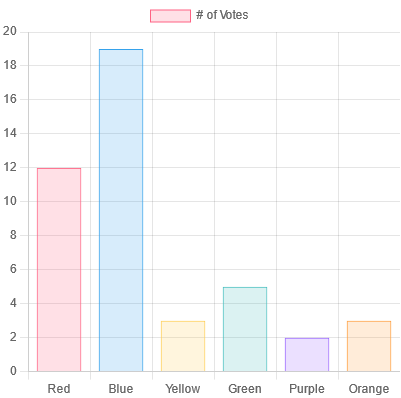
\includegraphics[height=8truecm]{images/chartjs-demo.png}
    \caption{Chart.js, egy Canvas API-t használó grafikont ábrázoló függvénykönyvtár. A betöltéskor az oszlopok automatikusan animálva vannak. Forrás: \cite{da2019learn}.}
    \label{fig:chart.js}
\end{figure}

\Section{Natív teljesítmény}

A JavaScript egy interpretált nyelv, amit a böngésző dolgoz fel. Mivel a böngésző egy univerzális futtatókörnyezet, így nem tud minden erőforrást a nyelv feldolgozására biztosítani. Segít az interpretáción a V8 JIT, ami bájtkódra (nem gépi kód) fordítja le a JavaScript kódunkat, ami ténylegesen fel tudja gyorsítani a futtatást, de a probléma attól még fennáll \cite{v8-jit}.

\Section{Már létező megoldások}
% TODO: Bővíteni

A probléma már egy évek óta fenntartó probléma, és már megoldás is született rá. A megoldást egy CrypticSwarm nevű GitHub felhasználó készítette el, de a megoldás már nem aktív 11 éve \cite{alt-xcbcanvas}.

A megoldás egy modul \textit{NodeJS}-ben. A technológia egy szintén ettől a felhasználótól származó másik technológia segítségével müködik. A XCB (pontosabban \textit{Cairo} (ami XCB-t használ UNIX rendszereken) hívásokat elérhetővé teszi JS-ben \cite{xcbjs}. Ennek a megoldásnak az előnye, hogy cross-platform és nem kell a rajzoló algoritmusokat újraimplementálni.